\documentclass[a4paper, 10pt]{article}
\usepackage[brazil]{babel}
\usepackage[utf8]{inputenc}
\usepackage{listings}
\usepackage{amsthm}


%\usepackage[pdftex]{graphicx}
%\graphicspath{{../pdf/}{../jpeg/}}
\usepackage{graphicx}


\title{Relatório do Laboratório 3}
\author{Felipe Bandeira da Silva}
\begin{document}
\maketitle
\lstset{language = Matlab}

%\section{Expansão em frações parciais}
 \newcounter{quest}
\begin{list}{\textbf{Questão \arabic{quest}.}}{\usecounter{quest}
\setlength{\labelwidth}{-2mm} \setlength{\parsep}{0mm}
\setlength{\topsep}{0mm} \setlength{\leftmargin}{0mm}}
\renewcommand{\labelenumi}{(\alph{enumi})}

\item Faça a expansão em frações parciais das funções abaixo com o auxílio do Matlab
e em seguida obtenha a transformada inversa de laplace.
    \begin{enumerate}
        \item       
            $$ 
                F(s) = \frac{10(s+2)(s+4}{(s+1)(s+3)(s+5)^2}
            $$

Usando a seguinte sequência de comandos para a obtenção da expansão,
            \begin{lstlisting}
a = [1 2];
b = [1 4];
num = 10*conv(a, b);
a = [1 1];
b = [1 3];
c = [1 5];
den = conv(conv(a, b), conv(c, c));
[r, p, k] = residue(num, den);

            \end{lstlisting}


        Resultado,

        \begin{lstlisting}
r = 
   -2.1875 
    3.7500
    1.2500
    0.9375

p = 
   -5.0000
   -5.0000
   -3.0000
   -1.0000

k = 
   []

        \end{lstlisting}
        Rearranjando os valores do resíduos, polos e termo de evidenciamento,

            $$
                F(s) = \frac{-2.1875}{s+5} + \frac{3.75}{s+5} + \frac{1.25}{s+3} + \frac{0.9375}{s+1}
            $$

            Aplicando a transformada inversa de laplace,

            $$
            f(t) = -2.1875 e^{-5t} + 3.75 e^{-5t} + 1.25 e^{-3t} + 0.9375 e^{-t}
            $$
         


    \item

        $$
        F(s) = \frac{s+1}{s(s^2+s+1)}
        $$

        Usando a mesma ideia usando no item (a) é possível obter, 

        \begin{lstlisting}
r = []
p = []
k = []
    \end{lstlisting}


    \item

        $$
        F(s) = \frac{2 s^3 + 5 s^2 + 3 s + 6}{s^3 + 6 s^2 + 11 s + 6}
        $$

        Usando a mesma ideia usando no item (a) é possível obter, 

        \begin{lstlisting}
r = 
   -6.0000
   -4.0000
    3.0000
p = 
   -3.0000
   -2.0000
   -1.0000
k = 
    2
    \end{lstlisting}


        Rearranjando os termos, 

        $$
        F(s) = \frac{-6}{s+3} + \frac{-4}{s+2} + \frac{3}{s+1} + 2
        $$

        Aplicando a transformada inversa de laplace,

        $$
        f(t) = -6 e^{-3t} -4 e^{-2t} + 3 e^{-t} + 2 \delta(t)
        $$

    \end{enumerate}











\item 
    Com base no sistema definido pela seguinte função de transferência, obtenha:

    $$
    G(s) = \frac{Y(s)}{X(s)} = \frac{3}{s(s+1)}
    $$
    \begin{enumerate}
        \item
            Função temporal $y(t)$ que representa a resposta do sistema quando excitado
            por um impulso unitário $x(t)=\delta(t)$ e rampa unitário $x(t)=r(t)$ \\

            O $\mathcal{L}(\delta(t)) = 1$ com isto é possivel obter a resposta 
            $Y(s)$ ao impulso, 
    
            $$
                Y(s) = \frac{3}{s(s+1)} \cdot 1
            $$

            Usando o comando "residue" para a expansão em frações parciais, temos,

            $$
                Y(s) = -\frac{3}{s+1} + \frac{3}{s}
            $$

            Aplicando $\mathcal{L}^{-1}$,

            $$
            \mathcal{L}^{-1}Y(s)=\mathcal{L}^{-1}( -\frac{3}{s+1} + \frac{3}{s} ),
            $$

            Resolvendo para $t$,

            $$
                y(t) = 3 - 3 e^{-t}
            $$\\

            

            Para o degrau unitário o $\mathcal{L}(u(t)) = \frac{1}{s}$, a resposta a excitação,

            $$
            Y(s) = \frac{3}{s(s+1)} \cdot \frac{1}{s} = \frac{3}{s^3+s^2}
            $$

            Expandindo em frações parciais,

            $$
            Y(s) = \frac{3}{s+1} - \frac{3}{s} + \frac{3}{s^2} 
            $$

            Aplicando $\mathcal{L}^{-1}$,

            $$
            y(t) = 3 - 3 t + 3 e^{-t}
            $$\\


            Para a ultima resposta, a $\mathcal{L}$ da rampa unitária é $\mathcal{L}(r(t)) = \frac{1}{s^2}$, logo,

            $$
            Y(s) = \frac{3}{s(s+1)} \cdot \frac{1}{s^2} = \frac{3}{s^4 + s^3}
            $$

            Expandindo em frações parciais,

            $$
            Y(s) = \frac{3}{s^3} - \frac{3}{s^2} + \frac{3}{s} - \frac{3}{s+1}
            $$

            Aplicando $\mathcal{L}^{-1}$,


            $$
            y(t) = \frac{3 t^2}{2} - 3 t + 3 - 3 e^{-t}
            $$

            \newpage
         \item 
             Apresente um um mesmo gráfico a resposta $y(t)$  obtida no item anterior, 
             considerando um intervalo de tempo de 0seg a 10seg com passo de 0.01seg.
 
             \begin{center}
                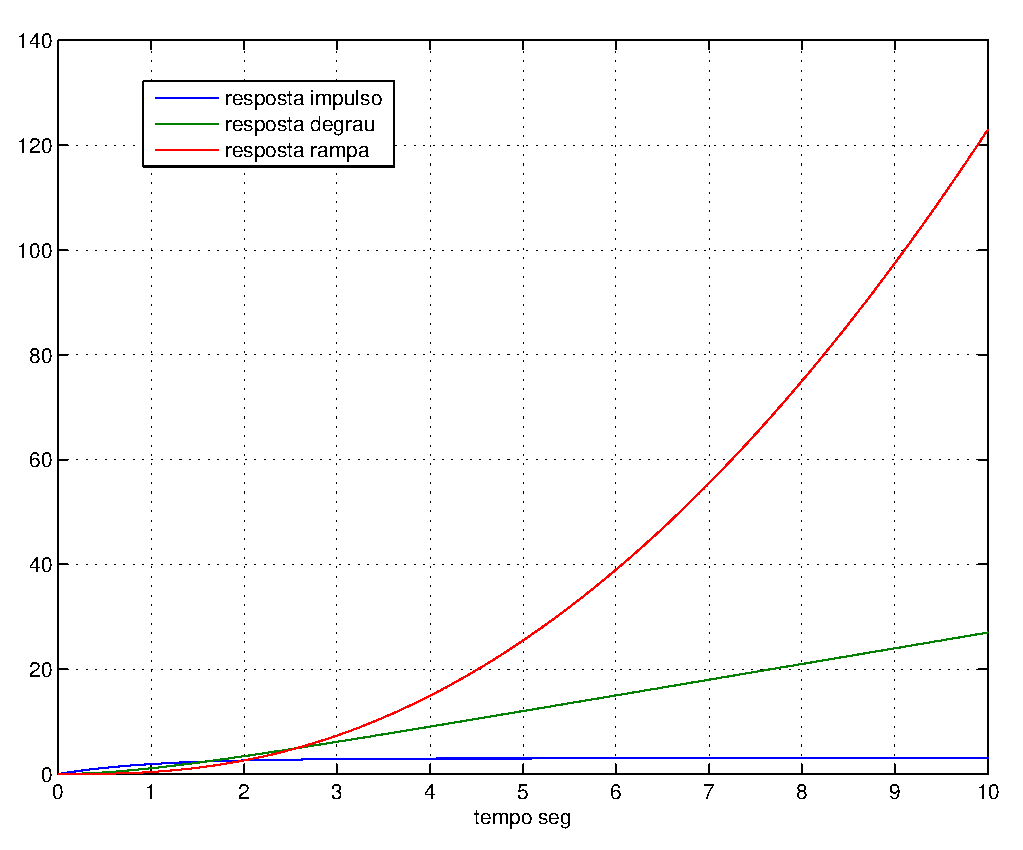
\includegraphics[scale=0.6]{fig2q.eps}
             \end{center}

             %\begin{figure}
             %   \centerline{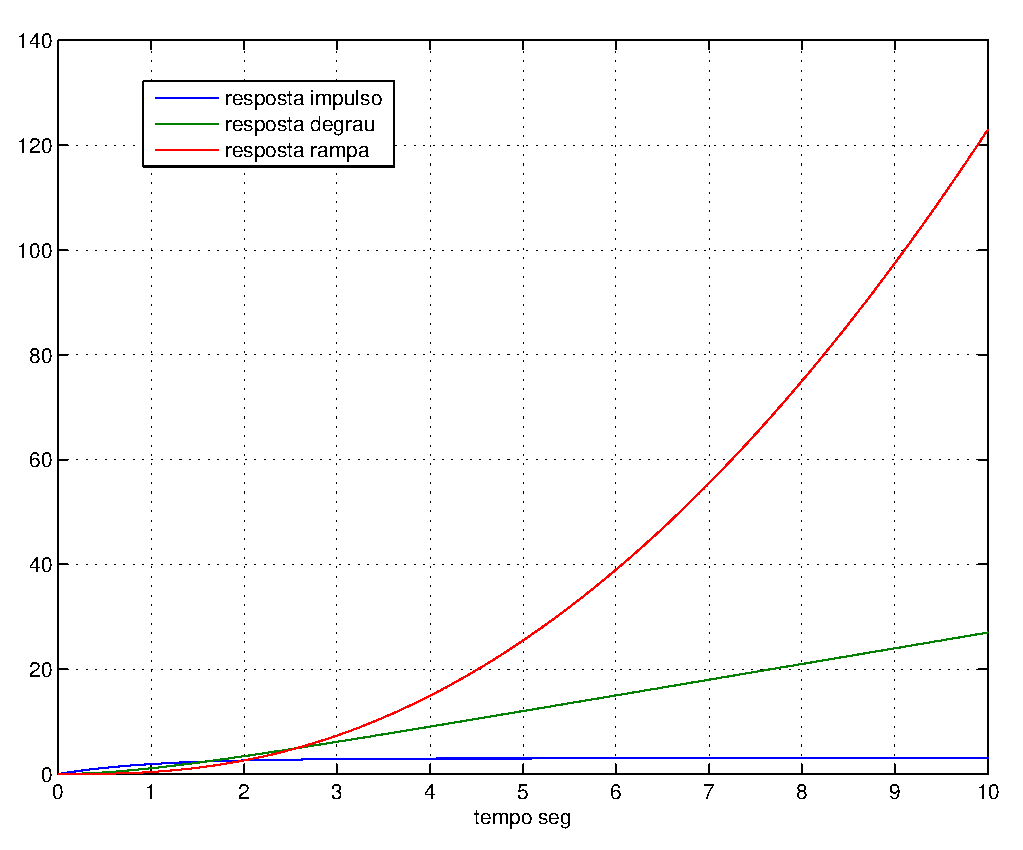
\includegraphics[scale=0.6]{fig2q.eps}
             %   \label{fig:TheFig}
             %   \caption{fefe}
             %\end{figure}

    \end{enumerate}

\newpage

\item
    Encontre os zeros, polos e ganho da função de transferencia abaixo. Em seguida, 
    represente e identifique os polos e zeros no plano-s.

    $$
    G(s) = \frac{4 s^2 + 16 s + 12}{s^4 + 12 s^3 +  44 s^2 + 48 s}
    $$


    Para a solução deste problema, criei o seguinte codigo,

 
     \begin{lstlisting}
num = [4 16 12];
den = [1 12 44 48 0];
z = roots(num);
p = roots(den);
k = 1;
fun = zpk(z, p, k);
     \end{lstlisting}

     Obtendo os pólos e zeros no plano-s,
        \begin{center}
                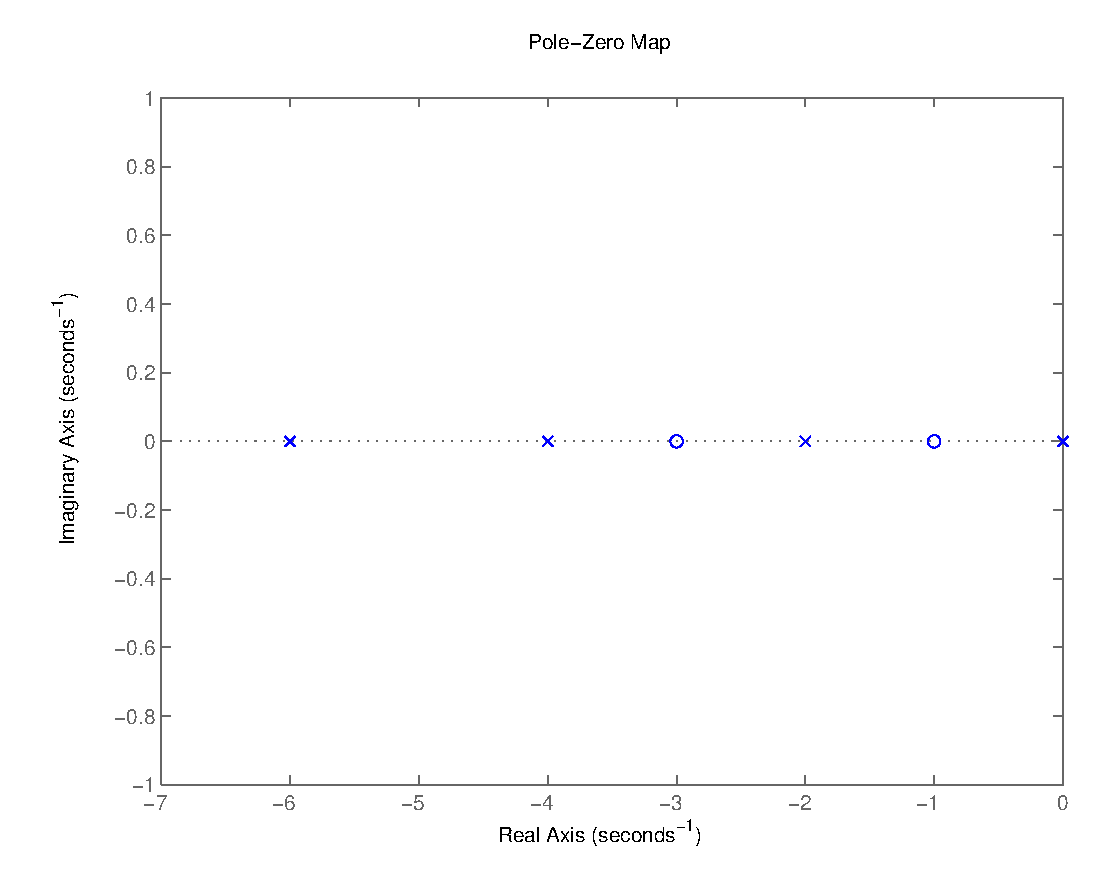
\includegraphics[scale=0.6]{fig3q.eps}
             \end{center}


\end{list}


\end{document}

